\documentclass[12pt]{article}

\usepackage{fontawesome}
\usepackage{hyperref}
\usepackage{xurl}
\usepackage{fancyvrb}
\usepackage{graphicx}
\usepackage{float}
\usepackage[tagged, highstructure]{accessibility}
\usepackage{bookmark}
\usepackage{enumitem}

\hypersetup{
    colorlinks=false,
    pdfborder={0 0 0},
    pdftitle={Password Cracking},
    pdfauthor={Adrianna Holden-Gouveia},
    pdfsubject={Information Security - Lab Assignment},
    pdflang={en-US},
    pdfkeywords={password cracking, John the Ripper, Kali Linux, dictionary attack, security}
}

% Configure PDF bookmarks for navigation
\bookmarksetup{
    numbered,
    open,
}

% Configure list spacing for better accessibility
\setlist{nosep}



\title{Password Cracking}
\author{
        Adrianna Holden-Gouveia \\
        Website: \href{https://aholdengouveia.name}{aholdengouveia.name}\\ 
        \date{\vspace{-5ex}}
        %Email: \href{mailto:admin@aholdengouveia.name}{admin@aholdengouveia.name} \\
%        \faLinkedin{: aholdengouveia} \\
        \faGithub {: aholdengouveia} \\
        \faTwitter {: aholdengouveia} \\
        }

%S\date{\today}


\begin{document}    

\maketitle

\section*{Accessibility Notice}
This document is also available in HTML format at:

Link: \href{https://aholdengouveia.name/InfoSec/labs/passwordcracking.html}{\textbf{\nolinkurl{https://aholdengouveia.name/InfoSec/labs/passwordcracking.html}}}

The HTML version provides enhanced accessibility features including keyboard navigation, screen reader support, responsive design, dark mode support, and high contrast options.


%\begin{abstract}
%This is a template for Linux Administration Lab work
%\end{abstract}
%\tableofcontents

\section*{Learning Outcomes}
By the end of this lab, you will be able to:
\begin{itemize}
    \item Explain how dictionary, hybrid, and brute force password attacks work
    \item Test password strength safely, using sample data in a virtual machine
    \item Compare how different hashing methods affect how well passwords are protected
    \item Recommend stronger password practices, and share them with others
\end{itemize}
\section*{Lab Instructions}

\subsection*{Screenshots}
Each screenshot should have your name, term, and year.  One of the easiest ways to do that is make a text document with your name and term/year on your computer and save it to use all term. Any screenshots that don't include this information won't be counted.

\begin{figure}[H]
    \centerline{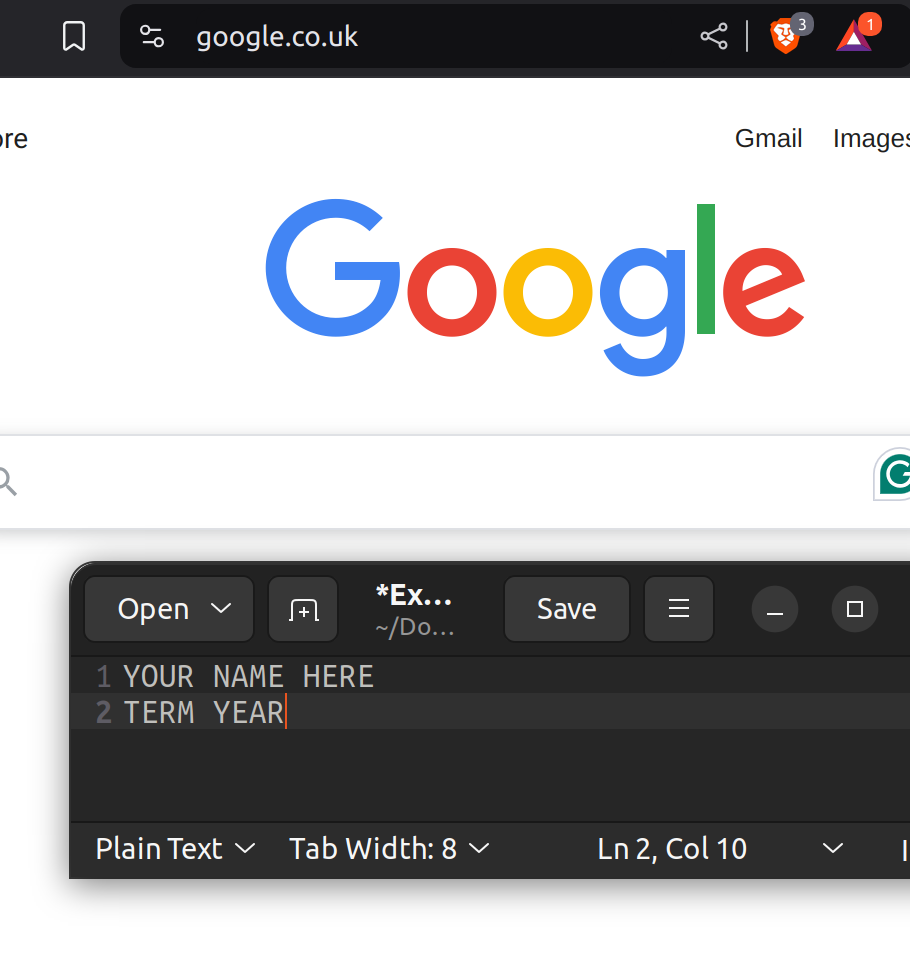
\includegraphics[scale=.2]{ExampleScreenshot.png}}
    \caption{This is an image of what each of your screenshots should look like}
    \alt{Example screenshot: a web browser showing the Google home page, with a small text editor window in front of it that says YOUR NAME HERE and TERM YEAR}
\end{figure}


\subsection*{This lab is about password cracking. You are going to use John the Ripper. This lab needs to be done through your Kali virtual machine}
First we're going to practice using Kali on a list of passwords I'm giving you, it's called "passwords.zip" and contains a file called "crack-these-please"
    \begin{enumerate}
        \item Download the "Passwords.zip  unzip. You need to make sure this file is unzipped and in your Kali virtual machine.  This should have 50 users with various passwords not in plain text.  Look at your unzipped crack-these-please file using cat, what's it look like?
        \item John the Ripper is a command line tool.  Check under "usage example" to see what this looks like when it's run Link: \href{https://www.kali.org/tools/john/}{\textbf{\nolinkurl{https://www.kali.org/tools/john/}}} If you run into any problems or need to troubleshoot go to John's homepage at Link: \href{https://www.openwall.com/john/}{\textbf{\nolinkurl{https://www.openwall.com/john/}}}
        \item A dictionary attack uses a word database, and tries it repeatedly. John the Ripper has this capability. Find one of the dictionaries included in Kali, either password.lst or RockYou,  Where did you find them? Dump the file's contents to the screen and then take a screenshot, use the command more.
        Press the spacebar, or hold it down, to make the display advance to the end of the file. You see that it is a list of potential passwords.
        \item Enter the following command to launch a dictionary attack:
        john --wordlist="dictionary" crack-these-please
        Where "dictionary" is the dictionary you've chosen, no quotes.
        Take a screenshot showing how many of the 50 passwords it was able to crack, what they are, and the time it took.
        \item John has created a list of solved passwords called john.pot.  Find that file and take a screenshot of that filed open.
        You see the same passwords you did before. But previously they were displayed along with the users who own them, now with their hashed versions. The hashed versions were the input to John's process; that's what got cracked.
        \item In default usage John the Ripper executes dictionary, hybrid, and bruteforce attacks in combination. Launch a combination attack by executing:
        john crack-these-please
        \item While john is working, examine the CPU utilization of your computer. Take a screenshot of it.
        \item Let John run long enough to do some more cracking. Note the time it took and how many additional passwords it was able to crack. Also note what the passwords are. The simpler ones should have been cracked in the earlier attempts, the ones that are being cracked now should be less simple passwords
        Getting all the passwords can take awhile, so if it is taking too long, you can hit CTRL-C to stop the run.
    \end{enumerate}
\subsection*{Making your own password file}
Kali includes a tool called htpasswd, which makes password files like the ones some websites use. If it isn't installed, install it with \texttt{sudo apt install apache2-utils}.

\textbf{Use only made-up passwords.} Never use a password you actually use, since you'll be sharing these files.

htpasswd options you'll need:
\begin{itemize}
    \item \texttt{-c} creates a new file. Only use it the first time. If you use it again, it replaces the file and erases the users you've already added.
    \item \texttt{-m} stores the password as an MD5 hash.
    \item \texttt{-s} stores the password as a SHA hash.
\end{itemize}

\begin{enumerate}
    \item Create the file and add your first user. Replace myfile and user1 with your own file name and username. It asks you to type the password twice.
\begin{Verbatim}
htpasswd -cm myfile user1
\end{Verbatim}
    \item Add more users to the same file, without \texttt{-c}:
\begin{Verbatim}
htpasswd -m myfile user2
\end{Verbatim}
    \item To use a SHA hash instead of MD5, use \texttt{-s} in place of \texttt{-m}:
\begin{Verbatim}
htpasswd -s myfile user3
\end{Verbatim}
    \item Check your file with \texttt{cat myfile}. Each line shows a username, and that user's password stored as a hash.
\end{enumerate}

\section*{Deliverables}
One file that includes your answers to the following, and all the screenshots requested in the lab:
\begin{enumerate}
    \item Write how many passwords you cracked, what they were and how long it took you from step 4. To show the passwords you have cracked in your files use the -show option with john.  Make sure you remember to pass john your password file. 
    \item Take a screen shot of your CPU utilization. With the hybrid attack, how many more passwords were you able to crack? What were they? How many of the cracked passwords contain varied combinations of letters, symbols, numerals, and case? Do the cracked passwords tend to be long or short? 
    \item Try running john -test What happened? What do you think this could be useful for?  What does your research say? Don't just guess what -test does
    \item  Using htpasswd try making a password file with only a single user, and use a dictionary word as the password.  Then make another file with the same user and password, but use MD5 hash. Then run a dictionary attack on both of them. Which one takes longer? Why do you think that is?
    \item Using htpasswd and a SHA and md5 option make a file of at least 10 usernames with passwords that are easy (12345) to difficult  (fjkwrhrT!@!) and switch with another student on the discussion board. Make sure to include at least 2 of each type.  
    \begin{itemize}
        \item Don't tell them your passwords.
        \item  Use John the Ripper to crack the password file they gave you
        \item Pass in the name of the student you switched with along with the file they gave you, how many passwords you were able to crack, which ones, and how long it took you.
        \item Include what you had to do differently to get more passwords (hint: did you have to change the --format to something else?)
    \end{itemize}
    \item Your report must include your passwords, the passwords you cracked and answers to all the questions asked in the lab and all screenshots requested.
\end{enumerate}
\section*{Resources}
References, a video, a PowerPoint and some notes are available at my website
Link: \href{https://www.aholdengouveia.name/InfoSec/Cryptography.html}{\textbf{\nolinkurl{https://www.aholdengouveia.name/InfoSec/Cryptography.html}}}

The sample file for this lab, passwords.zip
Link: \href{https://www.aholdengouveia.name/InfoSec/labs/passwords.zip}{\textbf{\nolinkurl{https://www.aholdengouveia.name/InfoSec/labs/passwords.zip}}}

John the Ripper on Kali
Link: \href{https://www.kali.org/tools/john/}{\textbf{\nolinkurl{https://www.kali.org/tools/john/}}}

John the Ripper homepage
Link: \href{https://www.openwall.com/john/}{\textbf{\nolinkurl{https://www.openwall.com/john/}}}

If you want to try something more (optional, not required for this class):

TryHackMe: Cryptography for Dummies, a free beginner room (free account needed)
Link: \href{https://tryhackme.com/room/cryptographyfordummies}{\textbf{\nolinkurl{https://tryhackme.com/room/cryptographyfordummies}}}

TryHackMe: Crack the Hash, a free practice room (free account needed)
Link: \href{https://tryhackme.com/room/crackthehash}{\textbf{\nolinkurl{https://tryhackme.com/room/crackthehash}}}

picoCTF practice challenges, free from Carnegie Mellon's CyLab Security Academy
Link: \href{https://cylabacademy.org/}{\textbf{\nolinkurl{https://cylabacademy.org/}}}

\end{document}